\subsection{Selected Exercises and Tools}\label{sec:selected_exercises}


\begin{figure*}[t!]

\centering
\begin{subfigure}[t]{0.3\textwidth}
  \centering
  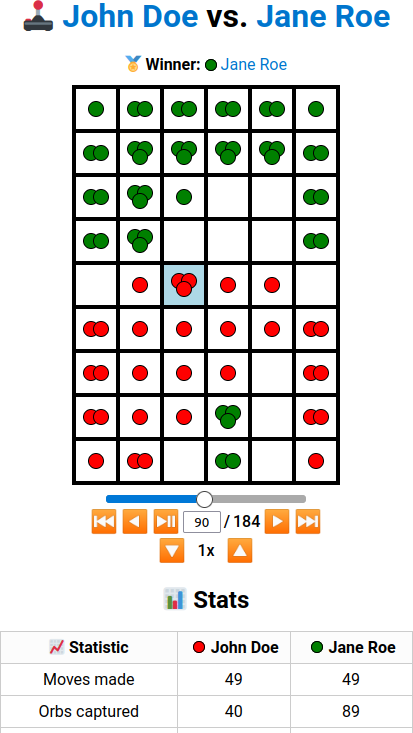
\includegraphics[width=\linewidth]{img/chainreaction.png}
  \caption{Game tournaments}
  \label{fig:chainreaction}
\end{subfigure}%
~
\begin{subfigure}[t]{0.3\textwidth}
  \centering
  
\includegraphics[width=\linewidth]{img/haskell_art.png}
  \caption{Art generation}
\end{subfigure}
~
\begin{subfigure}[t]{0.3\textwidth}
  \centering
  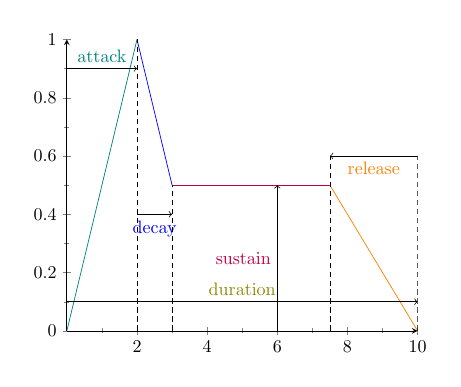
\begin{tikzpicture}[scale=0.65]
  \begin{axis}[
    minor tick num=1,
    samples=120,
    axis y line=left,
    axis x line=middle
    ]
    \addplot+[domain=0:10, mark=none, teal]
      coordinates {(0,0) (2, 1)};
    \addplot+[domain=0:10, mark=none, blue]
      coordinates {(2,1) (3, 0.5)};
    \addplot+[domain=0:10, mark=none, purple]
      coordinates {(3, 0.5) (7.5, 0.5)};
    \addplot+[domain=0:10, mark=none, orange]
      coordinates {(7.5, 0.5) (10, 0)};
    \addplot[densely dashed] coordinates {(2,0) (2,1)};
    \addplot[densely dashed] coordinates {(3,0) (3,0.5)};
    \addplot[densely dashed] coordinates {(7.5,0) (7.5,0.6)};
    \addplot[densely dashed] coordinates {(10,0) (10,0.6)};
    \addplot[->] coordinates {(0,0.9) (2,0.9)} node[midway, above, teal] {attack};
    \addplot[->] coordinates {(2,0.4) (3,0.4)} node[midway, below, blue] {decay};
    \addplot[->] coordinates {(6,0) (6,0.5)} node[midway,left, purple] {sustain};
    \addplot[<-] coordinates {(7.5,0.6) (10,0.6)} node[midway, below, orange] {release};
    \addplot[->] coordinates {(0,0.1) (10,0.1)} node[midway, above, olive] {duration};
  \end{axis}
  \end{tikzpicture}
  \caption{Music synthesis}
\end{subfigure}
\caption{Examples of exercises created as part of the course}
\end{figure*}

Many students at TUM have questioned the
applicability and usefulness
of functional languages after completing
the mandatory functional programming course.
We believe this is mainly due to two reasons:
\begin{enumerate*}[label=\arabic*)]
  \item introductory courses often stick
to simple algorithmic or mathematically inspired challenges and
\item side-effects (in particular I/O)
are often introduced rather late
in functional programming courses.
\end{enumerate*}

While we were able to introduce I/O midway through the course,
introducing it even earlier appeared difficult to us:
we think that students would be confused
if a ``special'' \mintinline{Haskell}{IO} type and \mintinline{Haskell}{do} notation were to
be introduced before they are comfortable
with the basic features of functional languages.
We thus focused on the other issue
and created exercises that go beyond
simple terminal applications.
Designing and implementing such exercises,
however, is labour-intensive.
As mentioned in \cref{sec:engagement},
we thus decided to reallocate resources and
let our student assistants help us with this work
rather than providing feedback for homework submissions.

This turned out to be a very fruitful idea:
the quality of our student assistants' work was often way above what we expected.
The one difficulty we faced was the mediocre quality of
tests written by most assistants
since they only had the rudimentary knowledge of QuickCheck taught as part of the course.
We thus hosted a workshop for them that explained
our testing infrastructure and best-practice
patterns when writing tests.
The quality of tests significantly increased following this workshop,
though we still had to polish them before publication.

We next introduce a few exercises and tools
that were created as part of the course.
They are available in this article's repository\footnote{\url{https://github.com/kappelmann/engaging-large-scale-functional-programming}},
next to our other exercises, including
a music synthesiser framework,
a turtle graphics framework,
an UNO framework,
and guided exercises for DPLL and resolution provers.
% Some further examples can be found on our competition blogs\footnote{\url{https://www21.in.tum.de/teaching/fpv/WS20/wettbewerb.html} (WS20) and
% \url{https://www21.in.tum.de/teaching/fpv/WS19/wettbewerb.html} (WS19)}.

\paragraph{Game Tournament Framework}
It has become a course tradition to run a game tournament over the Christmas break.
In this tournament, students are tasked with writing an AI for a board game that competes against the AIs of their fellow students.
To pass the homework sheet, it suffices to implement a basic strategy, but to score well in the competition, students came up with quite sophisticated strategies in past years.
The framework allows students to use statefulness and randomisation, so that there are few limits to the students' creativity.
% The best strategies usually use the minimax rule with alpha-beta-pruning and a clever evaluation function, which is particularly important in this setting because the game tree cannot be evaluated very far given the time limit for each submission in the tournament.

The tournament runs continuously for 2--3 weeks and the results are displayed on a website (see \cref{fig:chainreaction} for an example from WS20).
Students thus get reasonably quick feedback on how their strategy performs,
which keeps them engaged and allows them to improve their strategy iteratively.
The tournament became a popular feature of the course with 182 participating students in WS19 and 220 in WS20.

In our repository, we provide the framework along with code specific to the game from WS20, which is based on Chain Reaction\footnote{\url{ https://brilliant.org/wiki/chain-reaction-game/}}.
It runs a round-robin tournament,
collecting statistics for each game and player.
Instructions for adapting the framework to a different game can also be found in the repository.

\paragraph{Programming Contest Framework}\label{sec:contest}
To foster social interaction and diversify the bonus system,
we hosted an ACM-ICPC-like programming contest.
In such contests, students
participate in teams of 2--3,
solving as many programming challenges as possible in a given time frame,
and can check their ranking on a live scoreboard.
% At some point during the contest,
% the scoreboard gets frozen,
% and following the working time,
% solutions to all challenges are presented by the organisers.
% The final results are then revealed by unfreezing the scoreboard again.

We found existing solutions
to run such contests too complex for our purpose
and hence created a lightweight alternative.
Our framework continuously receives test results,
computes each team's score,
and displays the live scoreboard and task instructions on a website.
It is agnostic to the programming language and test runner used.
It expects tests results adhering to the Apache Ant JUnit XML schema,
but modifying it to support other formats is straightforward.
Deployment instructions can be found in this article's repository.

We ran an online iteration of the contest in WS20,
again using ArTEMiS as a test runner.
Teams were cooperating on their platform of choice
and were able to ask for clarifications on a dedicated online channel.
Our experiences are positive:
27 teams participated in the contest
and most stayed for the social hangout following it.
Using our framework,
the technical setup of the contest requires little time.
Some significant time, however,
must be spent on setting up the challenges,
tests, and solutions,
though plenty of them may be found
online by searching for other contests,
which one then may modify and reuse.
We recommend offering such contests
to programming course instructors in general.
% for every lecture concerned with programming concepts.

\paragraph{I/O-Mocking Library}
As discussed in \cref{sec:tech_setup_test}, we primarily use QuickCheck to automatically assess homework submissions.
This raises the question how monadic I/O in Haskell can be tested.
Since we do not want to actually execute the side effects that the submitted code produces,
the obvious solution is to use a mocked version of Haskell's \mintinline{Haskell}{IO} type.

A standard approach to mock \mintinline{Haskell}{IO}, which is put forward by packages such as \texttt{monad-mock}\footnote{\url{https://hackage.haskell.org/package/monad-mock}} and \texttt{HMock}\footnote{\url{https://hackage.haskell.org/package/HMock}}, is to first extract the side effects that are required for a certain computation into a new typeclass.
Since a typeclass allows multiple instantiations,
we can then provide one instantiation that actually executes the side effects on the machine
and another one that just modifies a mocked version of the environment.
For example, to implement a function that copies a file,
we need two operations:
one for reading a file and one for writing a file.
\begin{minted}{Haskell}
import qualified Prelude
import Prelude hiding (readFile, writeFile)

class Monad m => MonadFileSystem m where
  readFile :: FilePath -> m String
  writeFile :: FilePath -> String -> m ()
\end{minted}
The implementation is straightforward.
\begin{minted}{Haskell}
copyFile :: MonadFileSystem m => FilePath -> FilePath -> m ()
copyFile source target = do
  content <- readFile source
  writeFile target content
\end{minted}

Due to the definition of \mintinline{Haskell}{MonadFileSystem}, the instance for \mintinline{Haskell}{IO} is trivial.
The mocked version can be implemented as a map from file names to file contents wrapped by the \mintinline{Haskell}{State} monad transformer to make it mutable.
We omit this instantiation of \mintinline{Haskell}{MonadFileSystem} for brevity.
Testing \mintinline{Haskell}{copyFile} is now as simple as checking whether the state of the file system is as expected after executing the function.
An example that includes the instance \mintinline{Haskell}{MonadFileSystem (State MockFileSystem)} and a test can be found in the repository in \href{https://github.com/kappelmann/engaging-large-scale-functional-programming/tree/main/resources/io_mocking/typeclass}{resources/io\_mocking/typeclass}.
\begin{minted}{Haskell}
instance MonadFileSystem IO where
  readFile = Prelude.readFile
  writeFile = Prelude.writeFile

data MockFileSystem = MockFileSystem (Map FilePath String)
instance MonadFileSystem (State MockFileSystem) where
  readFile = ...
  writeFile = ...
\end{minted}

While this approach is sufficient for many use cases,
it lacks one important property: transparency.
More specifically, the code submitted by students must contain or import \mintinline{Haskell}{MonadFileSystem} and the signatures of terms that use \mintinline{Haskell}{IO} must be adapted.
This is especially problematic because the lecture introduces \mintinline{Haskell}{IO} without mentioning monads.
% which are only introduced towards the end of the course.
Other approaches to test I/O
face similar issues~\cite{iotest1,iotest2}.

Instead of modifying existing code,
we delay the mocking to the compilation stage.
We achieve this with a mixin that replaces the \mintinline{Haskell}{IO} module of a submission with a mocked version.
The mocked \mintinline{Haskell}{IO} type can be realised similarly to above mock file system.
However, to achieve full transparency,
we not only need a file system but also handles, such as standard input and output, as well as a working directory.

All these aspects of the machine state are summarised in the type \mintinline{Haskell}{RealWorld} as seen below.
Crucially, the type also contains a mock user,
represented by a computation of type \mintinline{Haskell}{IO ()},
which interacts with a student's submission;
that is, the user generates the input for and reads the output of the student's submission.
For brevity, we do not show the full type here.
\begin{minted}{Haskell}
data RealWorld = RealWorld {
  workDir :: FilePath,
  files :: Map File Text,
  handles :: Map Handle HandleData,
  user :: IO (),
  ...
}
\end{minted}
Again, this type is wrapped by the \mintinline{Haskell}{State} monad transformer as well as two additional transformers \mintinline{Haskell}{PauseT} and \mintinline{Haskell}{ExceptT} in order to form the mocked \mintinline{Haskell}{IO} type.
\begin{minted}{Haskell}
newtype IO a =
  IO { unwrapIO :: ExceptT IOException (PauseT (State RealWorld)) a }
\end{minted}

While the transformer \mintinline{Haskell}{ExceptT} simply adds I/O exceptions,
such as errors for insufficient permissions,
the purpose of \mintinline{Haskell}{PauseT} is not obvious.
To understand its role, consider the following simple program that reads the user's name and greets them.
\begin{minted}{Haskell}
module Hello where

main = do
 name <- getLine
 putStrLn $ "Hello " ++ name
\end{minted}
In a normal (non-mocked) execution of the program, the program blocks and waits for input when \texttt{getLine} is called.
If our mocked \mintinline{Haskell}{IO} type would only consist of a state monad,
all the input to the program would have to be passed in one monolithic unit.
However, programs may consume input multiple times.
We thus need a way to suspend the program every time a blocking operation is called and transfer control over to our mock user.
The mock user then reacts to the output of the program and generates the input that the program is waiting for.
When the user is done, it yields and the program of the student is resumed.

These considerations lead us to the monad below,
consisting of two operations:
The first one pauses execution and the second one runs a computation of the monad until either \texttt{pause} is called or the computation finishes.
In the former case,
\texttt{stepPauseT} returns a \mintinline{Haskell}{Left c} where \texttt{c} represents the rest of the computation, i.e.\ the part of the computation that is executed when resuming.
Otherwise, the final result \texttt{r} of the computation is returned as \mintinline{Haskell}{Right r}.
It should be noted that the pause monad is an instance of the more general coroutine monad as provided by the \texttt{monad-coroutine}\footnote{\url{https://hackage.haskell.org/package/monad-coroutine}} package.
For the implementation details of the corresponding monad transformer \mintinline{Haskell}{PauseT}, we refer to the repository.
\begin{minted}{Haskell}
class Monad m => MonadPause m where
  pause :: m ()
  stepPauseT :: m a -> m (Either (m a) a)
\end{minted}

We exemplify the mechanics of the mocking framework with a simple test of above \mintinline{Haskell}{main} function.
To this end, we first implement a mock user that takes a name and supplies it to the standard input of \mintinline{Haskell}{main}.
The user then reads the output of the program and checks whether it printed the expected greeting.
In the QuickCheck property \mintinline{Haskell}{prop_hello},
we evaluate the interaction between the mock user and the program with \mintinline{Haskell}{Mock.evalIO} on \mintinline{Haskell}{Mock.emptyWorld}, a minimal \mintinline{Haskell}{RealWorld} that contains no files and only the absolutely necessary handles: standard input, standard output, and standard error.
The interaction itself sets the user to \texttt{user s},
then executes the \mintinline{Haskell}{main} function, and finally runs the user to completion.
\begin{minted}{Haskell}
import qualified Mock.System.IO.Internal as Mock
import qualified Hello as Sub

user :: String -> Mock.IO ()
user s = do
  Mock.hPutStrLn Mock.stdin s
  output <- Mock.hGetLine Mock.stdout
  when (output /= ("Hello " ++ s))
    (fail $ "\nExpected:\n" ++ "Hello " ++ s
      ++ "\nActual:\n" ++ output ++ "\n")

prop_hello = forAll (elements ["Karl", "Friedrich", "Rosa"]) $ \s ->
  Mock.evalIO (Mock.setUser (user s) >> Sub.main >> Mock.runUser)
              Mock.emptyWorld
\end{minted}
\begin{figure}[t!]
  \centering
\scalebox{0.75}{
\begin{tikzpicture}[cnode/.style={draw,rectangle,minimum height=2.5em}, >=stealth]
  \node[cnode] (P1) {\lstinputlisting[style=Haskell]{sections/practical_part/io_mocking/P.hs}};
  \node[cnode, right=2cm of P1.south east, anchor=south west] (P2) {\lstinputlisting[style=Haskell,firstline=2]{sections/practical_part/io_mocking/P.hs}};
  \node[cnode, right=2cm of P2.south east, anchor=south west] (P3) {\texttt{()}};

  \path (P1.south east) -- coordinate (MP12) (P2.south west);
  \path (P2.south east) -- coordinate (MP23) (P3.south west);
  \node[cnode, below=2cm of MP12, anchor=north] (U1) {\lstinputlisting[style=Haskell]{sections/practical_part/io_mocking/U.hs}};
  \node[cnode, below=2cm of MP23, anchor=north] (U2) {\lstinputlisting[style=Haskell,firstline=4]{sections/practical_part/io_mocking/U.hs}};
  \node[cnode, right=2cm of U2.north east, anchor=north west] (U3) {\texttt{()}};

  \path (U2.east |- U3) -- coordinate (MU23) (U3);
  \path (P3 -| MU23) -- node[shape=circle, fill=black, scale=0.8] (END) {} (MU23);

  \begin{scope}[>=open triangle 45]
    \draw[->] (P1.east |- P2) -- node[above] {\texttt{Left}} (P2);
    \draw[->] (P2.east |- P3) -- node[above] {\texttt{Right}} (P3);
    \draw[->] (U1.east |- U2) -- node[below] {\texttt{Left}} (U2);
    \draw[->] (U2.east |- U3) -- node[below] {\texttt{Right}} (U3);
  \end{scope}

  \begin{scope}[>=triangle 45]
    \draw[->] (P1.east |- P2) to[out=0, in=90] (U1);
    \draw[->] (P2.east |- P3) to[out=0, in=90] (U2);
    \draw[->] (U1.east |- U2) to[out=0, in=-90, looseness=0.85] (P2);
    \draw[->] (U2.east |- U3) to[out=0, in=-90] (END);
  \end{scope}

\end{tikzpicture}
}
\caption{
  Interaction between the mock user and the student's submission.
  White arrows indicate the return value of \texttt{stepPauseT} and black arrows indicate transfer of control.
  The black dot signifies the end of the interaction.\label{fig:iomocking}
}
\end{figure}

\cref{fig:iomocking} illustrates the evaluation steps of \mintinline{Haskell}{Mock.evalIO}.
Note that there are two blocking operations (i.e.\ operations that call \texttt{pause} internally),
namely \texttt{getLine} and \mintinline{Haskell}{Mock.hGetLine Mock.stdout}.
When \mintinline{Haskell}{Mock.evalIO} encounters any such operation,
it transfers control between the user and the program as indicated by the black arrows.
Control is also transferred if the computation runs until completion without meeting a \texttt{pause}.
The horizontal axis with white arrows illustrates the return values of \texttt{stepPauseT}.
Focusing on \mintinline{Haskell}{main},
we see that \texttt{stepPauseT}
returns the remaining computation \mintinline{Haskell}{putStrLn $ "Hello " ++ x} wrapped in a \mintinline{Haskell}{Left}
when encountering \texttt{getLine}.
After the user provides the input for \texttt{getLine} and yields, the \mintinline{Haskell}{main} function prints the greeting and finishes with the result \mintinline{Haskell}{Right ()}.
Similarly, the user is blocked on \mintinline{Haskell}{Mock.hGetLine},
which means that the remaining computation only consists of the \texttt{when} check, which is executed as soon as \mintinline{Haskell}{main} is done.
This explains why we need to run \mintinline{Haskell}{Mock.runUser} after \mintinline{Haskell}{Sub.main} since the crucial \texttt{when} check would never be executed otherwise.

All in all, the mocking framework lets us uniformly test student submissions with common frameworks like QuickCheck and SmallCheck regardless of whether they contain I/O effects.



